\documentclass[10pt,a4paper,english]{article}
\usepackage{geometry,metalogo,hyperref,babel,mdwlist,array,multicol}
\usepackage[default,osf]{sourceserifpro}
\usepackage[scaled=.95]{sourcecodepro}

\hypersetup{
    colorlinks,
    citecolor=blue,
    filecolor=blue,
    linkcolor=blue,
    urlcolor=blue
}
\newcommand*\file[1]{\href{run:#1.pdf}{#1}}

\title{\bfseries
	\Huge sourceserifpro\\
	\Large Adobe's Source Serif Pro typeface for \LaTeX
}

\author{Silke Hofstra, \href{mailto:tex@slxh.nl}{tex@slxh.nl}}
\date{Documentation for sourceserifpro v1.1.\\ \today}

\begin{document}
\maketitle
\begin{multicols}{2}
This package provides the Source Serif Pro font in an easy to use way. For \XeLaTeX\ and \LuaLaTeX\ users the original OpenType fonts from \href{https://github.com/adobe-fonts/source-serif-pro}{GitHub} are used. The entire font family is included.

This package is also available on \href{https://github.com/silkeh/latex-sourceserifpro}{GitHub}.

\section{Options}
The package has the following options:
\begin{itemize*}
	\item \textbf{oldstyle, osf}:  use old style numbers.
	\item \textbf{lining, nf, lf}: use lining numbers.
	\item \textbf{tabular}:        use fixed-width numbers.
	\item \textbf{proportional}:   use normal numbers.
	\item \textbf{black}:          \texttt{\textbackslash bfseries} is black.
	\item \textbf{semibold}:       \texttt{\textbackslash bfseries} is semibold.
	\item \textbf{bold}:           \texttt{\textbackslash bfseries} is bold.
	\item \textbf{light}:          \texttt{\textbackslash mdseries} is light.
	\item \textbf{extralight}:     \texttt{\textbackslash mdseries} is extra light.
	\item \textbf{regular}:        \texttt{\textbackslash mdseries} is regular.
	\item \textbf{scale, scaled}:  Change the scaling with a factor. For example:  \texttt{scale=.5}
	\item \textbf{default}:        Source Serif Pro is set as the default font family.
	\item \textbf{normdefault}:    Source Serif Pro is not set as the roman (serif) family.
	\item \textbf{type1, t1}:      Override automatic detection and use the Type 1 fonts.
	\item \textbf{opentype, otf}:  Override automatic detection and use OpenType fonts.
\end{itemize*}
The following options are enabled by default: lining, proportional, bold and regular.

\section{Commands}
Commands for all weights are also provided for \XeLaTeX\ and \LuaLaTeX\ users.
\begin{itemize*}
	\item \texttt{\bfseries \textbackslash sourceserifpro}
		-- the regular and bold weights.
	\item \texttt{\bfseries \textbackslash sourceserifprolight}
		-- the light and semibold weights.
	\item \texttt{\bfseries \textbackslash sourceserifproextreme}
		-- the extra light and black weights.
\end{itemize*}

\section{Licence}
Adobe's Source Serif Pro typeface is available under the \href{http://scripts.sil.org/OFL}{SIL Open Font License 1.1}.\\
All \LaTeX\ code is available under the \href{http://www.latex-project.org/lppl/}{\LaTeX\ project public license} v1.3 or later.

\section{Specimen}
Simple specimen can be found on page \pageref{sec:specimen}. Full specimen can be \href{http://store1.adobe.com/type/browser/pdfs/1966.pdf}{acquired from Adobe}.

\section{OpenType}
The OpenType fonts have many features, including old style numerals (1 6 9) and ligatures (fi fl ft).

\subsection{Features}
A complete list of available font features is available on page \pageref{sec:otfinfo}. More information on how to use font features can be found in the \href{http://mirror.ctan.org/macros/latex/contrib/fontspec/fontspec.pdf}{fontspec documentation}.

\subsection{Files}
\begin{itemize*}
	\item SourceSerifPro-Black.otf
	\item SourceSerifPro-ExtraLight.otf
	\item SourceSerifPro-Regular.otf
	\item SourceSerifPro-Bold.otf
	\item SourceSerifPro-Light.otf
	\item SourceSerifPro-Semibold.otf
\end{itemize*}

\section{Type1}
The following Type1 font families are included:
\begin{itemize*}
	\item SourceSerifPro-LF
	\item SourceSerifPro-TLF
	\item SourceSerifPro-OsF
	\item SourceSerifPro-TOsF
\end{itemize*}
With series ‘el’, ‘l’, ‘m’, ‘sb’, ‘b’, ‘k’ and shape ‘n’.

\section{Version history}
\subsection*{1.1}
\begin{itemize*}
	\item Updated package with fonts 1.017
\end{itemize*}

\subsection*{1.0}
\begin{itemize*}
	\item Initial release with fonts 1.014
\end{itemize*}

\section{Known issues}
\begin{itemize*}
	\item There are no known issues.
\end{itemize*}
\vspace{0pt plus 1filll}\mbox{}
\newpage
\end{multicols}

\section{Specimen}
\label{sec:specimen}
\subsection{OpenType}
\begin{figure}[ht]
	\centering
	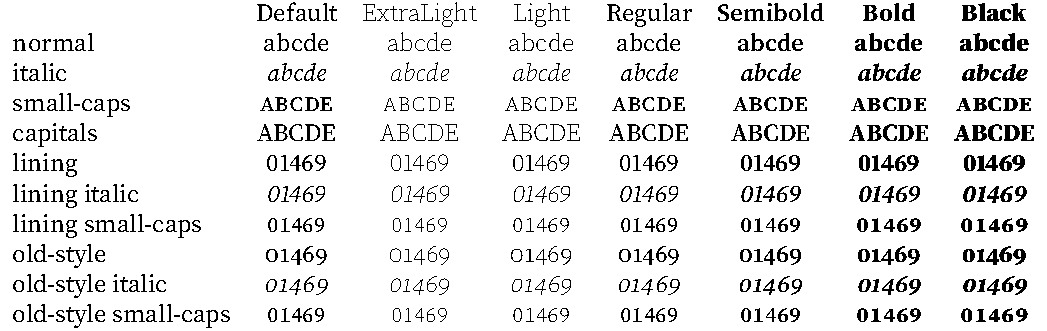
\includegraphics{sourceserifpro-otf-specimen}
\end{figure}
This table can also be found in \file{sourceserifpro-otf-specimen}.

\subsection{Type1}
\begin{figure}[ht]
	\centering
	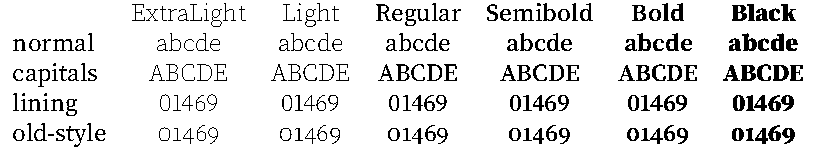
\includegraphics{sourceserifpro-type1-specimen}
\end{figure}
This table can also be found in \file{sourceserifpro-type1-specimen}.

\newpage
\section{Opentype features}
\label{sec:otfinfo}

\begin{figure}[ht]
	\centering
	\begin{tabular}{>{\ttfamily}l l}
		aalt & Access All Alternates \\
		case & Case-Sensitive Forms \\
		dnom & Denominators \\
		frac & Fractions \\
		kern & Kerning \\
		liga & Standard Ligatures \\
		lnum & Lining Figures \\
		numr & Numerators \\
		onum & Oldstyle Figures \\
		ordn & Ordinals \\
		pnum & Proportional Figures \\
		sinf & Scientific Inferiors \\
		size & Optical Size \\
		subs & Subscript \\
		sups & Superscript \\
		tnum & Tabular Figures \\
		zero & Slashed Zero \\
	\end{tabular}
\end{figure}
\textit{(list generated with otfinfo)}

\end{document}

